\section{Results}\label{sec:results}
\paragraph{Positive controls.} Our nearest neighbour reproduces MCTS-AHD's published
``Greedy Construct'' objectives on all three test sets: 6.959, 9.706 and 13.461. Our LKH means
reproduce its published optima at $n=50$ and 100 (5.6755 and 7.7680). At $n=200$ they do not
(10.708 against 10.659), which we examine at the end of this section. All gaps below are against our
reference.

\begin{table*}[t]\centering\small
\caption{Gap to the optimum (\%) and median wall seconds per instance on MCTS-AHD's released test sets
(1,000 instances each unless the count is given). \emph{Emitted}: a \code{select\_next\_node} that builds one tour from the distance matrix (a function of its arguments) and returns its next node; greedy and LKH cache the plan per instance, and the uncached row gives the cost without it.
Published rows are as printed. Times come from one shared, loaded laptop; read them as orders of
magnitude.}\label{tab:main}
\begin{tabular}{@{}llrrrrrr@{}}\toprule
& & \multicolumn{2}{c}{$n=50$} & \multicolumn{2}{c}{$n=100$} & \multicolumn{2}{c}{$n=200$}\\
\cmidrule(lr){3-4}\cmidrule(lr){5-6}\cmidrule(l){7-8}
Method & kind & gap & s & gap & s & gap & s\\\midrule
LKH, emitted (ceiling) & classical & 0.00 & 0.015 & 0.00 & 0.056 & 0.00 & 0.27\\
\textbf{Greedy edge + 2-opt + Or-opt, emitted} & classical & \textbf{1.85} & 0.015 & \textbf{2.44} & 0.045 & \textbf{2.85} & 0.13\\
\quad same, without the cache & classical & 1.85 & \NoCacheRow & 2.44 & \NoCacheRowH & 2.85 & \NoCacheRowT\\
Farthest insertion (1977), emitted & classical & 5.53 & 0.046 & 7.49 & 0.24 & 9.03 & 1.0\\
Nearest neighbour & classical & 22.62 & 0.0004 & 24.94 & 0.001 & 25.71 & 0.006\\\midrule
TIDE, appendix heuristic (transcribed) & LLM, re-run & 3.02 & 3.3 & 6.21 & 46 & \TideGap & \TideSec\\
& & \footnotesize(200 inst.) & & \footnotesize(30 inst.) & & \footnotesize(\TideN\ inst.) &\\
MCTS-AHD, released & LLM, re-run & 8.78 & 0.72 & 10.30 & 3.5 & \MctsGap & \MctsSec\\
& & & & & & \footnotesize(\MctsN\ inst.) &\\
HiFo-Prompt, released & LLM, re-run & 9.09 & 4.4 & \HifoGapH & \HifoSecH & \HifoGap & \HifoSec\\
& & & & \footnotesize(\HifoNH\ inst.) & & \footnotesize(\HifoN\ inst.) &\\
ReEvo, released & LLM, re-run & 10.46 & 0.021 & 11.87 & 0.15 & 13.01 & 0.96\\
AEL, released & LLM, re-run & 10.30 & 0.036 & 12.26 & 0.15 & 14.07 & 0.94\\
RefineEvo, released file & LLM, re-run & 11.71 & 0.071 & 12.65 & 0.34 & 13.76 & 1.9\\
Clade-AHD, released file & LLM, re-run & 22.62 & 0.001 & 24.94 & 0.004 & 25.71 & 0.015\\\midrule
TIDE~\cite{tide} & published & 4.76 & -- & 7.15 & -- & 10.65 & --\\
SimpleEvol~\cite{simpleevol} & published & 4.77 & -- & 6.47 & -- & 9.49 & --\\
HiFo-Prompt~\cite{hifo} & published & 6.63 & -- & 8.58 & -- & 8.88 & --\\
PathWise~\cite{pathwise} & published & 8.41 & -- & 11.85 & -- & 12.14 & --\\
MCTS-AHD~\cite{mctsahd} (GPT-4o-mini) & published & 9.69 & -- & 11.79 & -- & 13.71$^\dagger$ & --\\
MoH~\cite{moh} & published & 9.89 & -- & 11.44 & -- & 13.31 & --\\
CALM~\cite{calm} & published & 10.04 & -- & 11.58 & -- & 13.41 & --\\
Clade-AHD~\cite{clade} & published & 10.39 & -- & 9.22 & -- & 11.30 & --\\\bottomrule
\multicolumn{8}{@{}l}{\footnotesize $^\dagger$13.19 against the corrected optimum. Published rows use each paper's own test sets and references; see the repository's literature notes.}
\end{tabular}\end{table*}

\begin{figure*}[t]\centering
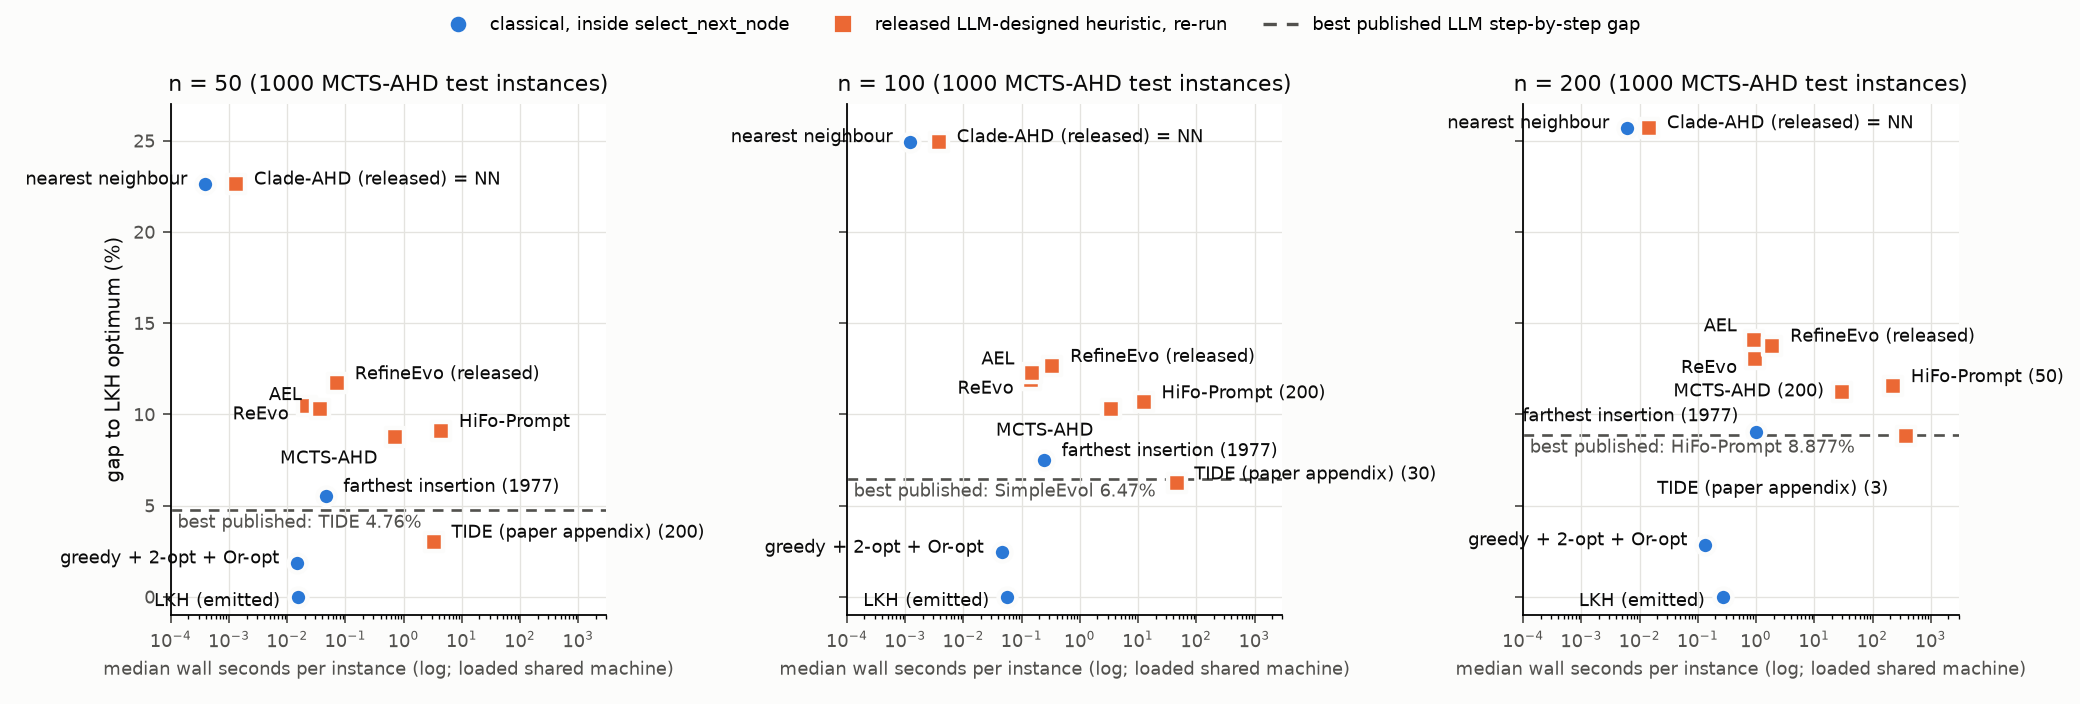
\includegraphics[width=\textwidth]{fig_pareto.png}
\caption{Gap against time per instance on MCTS-AHD's test sets. Blue: classical methods inside
\code{select\_next\_node}. Orange: released LLM-designed heuristics, re-run on the same instances and
machine. Dashed: best published step-by-step result. Classical methods occupy the whole lower-left
frontier.}\label{fig:pareto}
\end{figure*}

\paragraph{The interface's ceiling (H1).} Table~\ref{tab:main} and Figure~\ref{fig:pareto} show the
main result. Emitting a greedy-edge tour improved by 2-opt and Or-opt beats every published step-by-step result at every size (RedAHD, which drops the per-step interface, reports 1.62\% at $n=50$): 1.85\% against TIDE's 4.76\%, 2.44\% against SimpleEvol's
6.47\%, and 2.85\% against HiFo-Prompt's 8.88\%. It also beats RefineEvo's Claude Opus heuristic,
whose published objectives imply about 3.3\% and 4.7\% at $n=100$ and 200, and TIDE's own heuristic
re-run on the same instances. An emitted LKH tour reaches the reference. The benchmark therefore
does not bound what a \code{select\_next\_node} can achieve. It only bounds what the LLM search
chose to write.

\paragraph{A 1977 baseline (H3).} Farthest insertion, a one-pass construction with no local search and no cache, beats every LLM-AHD row of MCTS-AHD's Table~1 and of CALM, MoH, Clade-AHD and PathWise at every size (those tables also list POMO, a trained neural solver, which is not part of the comparison).
Against the released MCTS-AHD heuristic re-run on the same 1,000 instances at $n=50$, it is shorter
by 0.184 per instance (95\% CI $[-0.202,-0.167]$; 735 wins, 265 losses), and its CIs against
MCTS-AHD, ReEvo and AEL are below zero at every size. On MCTS-AHD's own TSPLIB protocol (the 14
instances in its repository), farthest insertion averages 8.70\% against MCTS-AHD's 11.17\% and
Christofides' 11.21\%. Greedy + 2-opt + Or-opt averages 2.38\% there. Even nearest neighbour with plain 2-opt (5.88 / 6.94 / 7.75\%) beats every LLM-AHD row of the MCTS-AHD lineage.

\paragraph{Released heuristics are Pareto-dominated (H2).} \HtwoSentence\ The exception is
Clade-AHD's released \code{gpt.py}. Its score is $0.5d - 1/(d+10^{-5})$ plus a constant, where $d$ is
the distance from the current node; this is increasing in $d$, so it always picks the nearest node,
and it reproduces nearest neighbour's tour on every instance. Nothing can be strictly faster and
better than it. HiFo-Prompt's released heuristic averages eight ``lookahead simulations'' that are
the same deterministic rollout; one gives identical tours, 6.9$\times$ faster. \NoCacheHtwo\ To give the LLMs their due, MCTS-AHD's blend (0.7 immediate distance, 0.3 rollout, plus a centre penalty) beats a textbook
nearest-neighbour rollout (8.78\% against 10.82\%).

\paragraph{Robustness (H4).} \HfourSentence

\paragraph{The $n=200$ reference.} MCTS-AHD's Table~1 lists 10.659 as the optimal mean at $n=200$.
On its released test200, the instances that reproduce its nearest-neighbour objective exactly, our LKH mean is 10.708, and the evidence says it is the optimum:
\begin{itemize}
\item our LKH setting matched MCTS-AHD's heavier LKH setting on 20 of 20 instances;
\item an integer program (HiGHS with subtour cuts) proved our tours optimal on 5 of 5 instances;
\item PathWise independently reports 10.709 on its own 250 instances.
\end{itemize}
Gaps computed against 10.659 are therefore overstated by about 0.5 points: MCTS-AHD's 13.71\% is
13.19\%. SimpleEvol and CALM print the same 10.659 as their reference, and Clade-AHD's $n=200$ numbers imply it. At $n=50$ and 100 the published
references are correct.
